\section{Kravinsamlingsmetoder - Daniel Falk}
\subsection{Inledning}
Jag har i detta projekt haft rollen som analysansvarig vilket innebär en analys av kundens behov och framställning av krav utifrån dessa. Denna enskilda del beskriver vilka kravinsamlingsmetoder och verktyg som använts för att ta fram krav. Erfarenheterna används för att undersöka om metoderna och verktygen kan användas för att tillfredsställa kundens verkliga behov.
\subsubsection{Syfte}
Syftet med denna del av rapporten är att undersöka olika metoder och verktyg för kravframställning. Fokus ligger på intervjuer, observationer och prototyper. Rapporten går speciellt in på hur prototyper använts för att ta fram, testa och validera krav i detta projekt.
\subsubsection{Frågeställning}
%Hur kan man samla in krav som tillfredställer kundens verkliga behov?
\begin{itemize}
\item Är intervjuer och observationer bra metoder för att analysera kundens behov?
%\item Hur kan intervjuer och observationer användas för att analysera kundens behov?
\item Hur kan man arbeta med prototyper för att framställa krav?
\item Hur kan man använda prototyper för att testa och validera krav?
\end{itemize}
\subsubsection{Avgränsningar}
Rapporten har sin utgångspunkt i hur kravframställningen gått till i detta projekt och gör inga jämförelser med andra kravinsamlingsmetoder. Metoden bör inte ses som ett allmänt tillvägagångssätt.
\subsection{Bakgrund}
Att förstå kundens verkliga behov utgör grunden för ett lyckat projekt. Ett projekt faller ofta på grund av ofullständiga krav \cite{Hull}.
För att samla in krav kan flera olika metoder och tekniker användas. Metoderna kan variera och vara olika bra på att fånga upp olika typer av krav.
\subsection{Teori}
Teorin beskriver kravinsamlingsmetoder och  verktyg som använts i detta projekt. %och vilka problem som kan uppstå vid kravframställning. 
%\subsubsection{Problem}
%Skriv om och flytta till bakgrund
%Det finns ett antal barriärer som kan uppstå vid kravframställning. Ett problem är ofta att kunden inte kan formulera vad de vill ha. De kan se problemet men inte vad som behöver göras. De kan överdriva vissa problem medan andra förbises. 
%Ett annat problem är att kunden kan ha fastnat i ett invant mönster. De kan ha svårt att föreställa sig nya sätt att utföra en uppgift på.
%\cite{Lauesen} %Kolla upp om denna parafras är ok.

\subsubsection{Prototyper}
Prototyp är ett ord som har sina rötter i grekiskan och betyder \textit{första form} \cite{Arvola}. Deras syfte är att i ett tidigt skede beskriva hur det färdiga systemet ska fungera. Prototyper kan användas för att testa olika ideér och designer och kan variera i detaljrikedom. En tydlig skillnad är den mellan enkla LoFi-prototyper skissade på papper och datorbaserade HiFi-prototyper som mer liknar det riktiga systemet. LoFi-prototyper är ett bra verktyg för att snabbt kunna diskutera ett designval då det kräver väldigt lite arbete. En styrka hos LoFi-prototyper är att användare har lätt att komma med kritiska kommentarer utan att känna att de förolämpar designern \cite{Arvola}.
Prototyper kan vara temporära eller evolutionära \cite{Arvola}. En temporär prototyp är en prototyp som slängs efter att man har använt den och utvärderat den. En evolutionär prototyp slängs inte utan byggs vidare på. Man kan se det som en tidig version av det slutgiltiga systemet.

\subsubsection{Intervjuer}
%För att samla in krav kan flera olika metoder och tekniker användas. Metoderna kan variera och vara olika bra på att fånga upp olika typer av krav.
%Intervjuer
Intervjuer är en bra teknik för att få information om det nuvarande arbetet inom området och problem relaterade till det. Det är också bra för att få fram de stora målen med ett projekt. Många ser det som den huvudsakliga insamlingstekniken. De ger mycket information men för att lösa kritiska problem behövs ofta andra tekniker för att komplettera intervjuer \cite{Lauesen}. 
\subsubsection{Observationer}
Observationer är ett bra verktyg för att få information om nuvarande system eller arbetssätt. Det är ett bra sätt att komplettera intervjuer då användare ofta har svårt att förklara vad de verkligen gör \cite{Lauesen}. 
%(task demonstration)
%(scenarios)
 
\subsection{Metod}
Denna del beskriver hur intervjuer, observationer och prototyper har använts som metoder för kravframställning i detta projekt. Metoden beskriver också hur systemet testats för att validera och testa kraven. Frågeställningarna besvaras utifrån denna erfarenhet.
%Denna del beskriver hur kravframställningen gått till i detta projekt. Först beskrivs arbetet med att analysera kundens behov under förstudien. Vidare beskrivs mer ingående vilka metoder som använts och hur kraven valdes att representeras. Avslutningsvis beskrivs vilka användartester som genomfördes och hur dessa bedrog till utvecklingen.
%\subsubsection{Förstudie}
%Den största delen utav analysarbetet skedde under förstudien. Här identifierades de olika intressenterna och en kravspecifikation utarbetades. Våran första kontakt med projektet var en projektbeskrivning där kunden formulerade sina mål och visioner av projektet. Några vikta krav gavs också såsom att prototypdesign skulle genomföras i samarbete med kunden. Ett första möte utav fyra under förstudien gav sedan mer information och vi började våran kravinsamling. Vi kunde konstatera att vi hade två olika intressenter att arbeta med. Dels sjuksköterskorna som är användare av systemet och dels CMIT, Centrum för medicinsk teknik och IT, som ansvarar för sjukhusets IT-miljöer. För att förstå användarnas behov hölls ett studiebesök där vi fick en visning av nuvarande system och hur det används. Detta var nödvändigt för att verkligen förstå vad det var som behövde göras och vad som kunde förbättras. Från CMIT:s sida hölls mer tekniska möten där teknikval diskuterades. Här var det viktigt att ta reda på vilka begränsningar som fanns och vilka val som passade våra och deras erfarenheter.
\subsubsection{Intervjuer}
Möten med kund har genomförts vilka kan ses som intervjuer. Dessa möten har skett dels med IT-ansvariga, verksamhetsutvecklare och sjuksköterskor. För att samla in krav under dessa möten har vi dels fört anteckningar på papper eller dator och dels spelat in på mobil. När vi varit flera personer på möten har vi gått igenom och diskuterat våra anteckningar i efterhand. Vid oklarheter har vi antecknat dessa för att förtydliga med kund. Inspelning användes främst vid första mötet och var användbart då vi fick mycket information att sätta oss in i. 
%Kravspecifikationen skrev i Google docs. Detta valdes eftersom kraven utarbetades tillsammans med kund. Ett gemensamt redigerbart dokument gav en möjlighet för oss att arbeta på olika platser under kravframställningen vilket var effektivt. En kommentarsfunktion gav oss möjligheten att kommentera krav och föreslå förbättringar. Under interna möten och kundmöten var den gemensamma redigeringen också till nytta då kravformuleringar snabbt kunde genomföras.

%\subsubsection{Kravrepresentation}
%Kraven gavs en prioritetsordning för att kunna urskilja de mest väsentliga kraven. Detta kändes nödvändigt då vi var begränsade av en tidsbudget. En prioritering av kraven gav utrymme för vidareutveckling i mån av tid. Krav med prioritet 1 var att betrakta som grundkrav som skulle genomföras för att projektet skulle ses som godkänt. Krav med prioritet 2 var att betrakta som önskvärda och som skulle genomföras om då grundkraven var genomförda. Krav med prioritet 3 var krav som fångats upp med som skulle ses som framtida utbyggnad. 
%Koppla till nån litteratur/standard.

%Strukturering av krav
%Kraven numrerades för att lätt kunna refereras till under projektets gång. De delades också in i olika sektioner efter deras del i systemet. Sektionerna var plocklistor, handböcker, kartotek, lagersystem. En extra sektion för generella krav användes. Denna uppdelning kändes naturlig för detta projekt. 
%Man skulle också kunna dela in dem efter blablabla...

%Kravspecifikationen skrevs med stöd från standarden IEEE 830. Enligt standarden ska ett krav vara korrekt, otvetydigt, färdigt, konsekvent, prioriterat, verifierbart, modifierbart och spårbart. Detta eftersträvades men det kan diskuteras om alla krav passerar dessa filter. I slutändan var det ändå våran gemensamma förståelse för kravet tillsammans med kunden som accepterades. 

%Enligt standarden uttrycktes kraven på ska-form. Ett exempel på ett krav från projektet är följande: "Plocklistor ska innehålla information om artikelns namn, förråd, sektion, hylla och fack".

\subsubsection{Observationer}
För att få en inblick i hur operationsförberedelserna fungerar i dagsläget genomfördes ett studiebesök på sjukhusets operationsavdelning. Vi fick här se problemet ur sjuksköterskornas synvinkel. Vi fick se hur man arbetade i artikellagret i dagsläget vilket var nödvändigt för att kunna genomföra en förbättring. De svårigheter som beskrivits blev tydligare och det blev lättare att föreställa sig en lösning på problemet.

\subsubsection{LoFi-prototyper}
Under förstudien valde vi att vid två tillfällen göra LoFi-prototyper som vi tog med till kund. Vid dessa tester kunde vi se om vi var på rätt bana när det gällde design och struktur. LoFi-protptyperna utjordes av enkla pappersskisser. Ett exempel visas i figur~\ref{fig:lofiprototyper}.
\begin{figure}[htbp]
\begin{center}
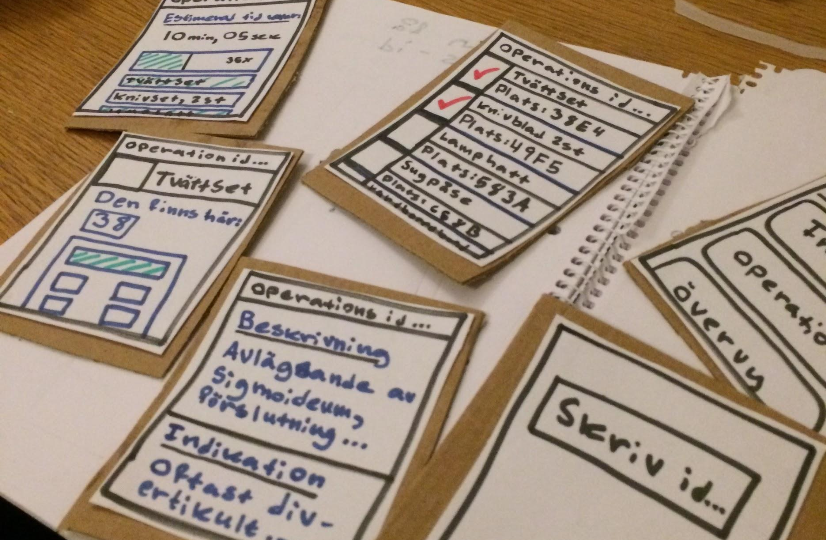
\includegraphics[scale=0.2]{lofiprototyper.png}
\caption{LoFi-prototyper}
\label{fig:lofiprototyper}
\end{center}
\end{figure}
Det första tillfället fokuserade på gränssnittsdesign och navigation i systemet. Prototyperna visades för en sjuksköterska som fick föreställa sig systemet. De olika korten gicks igenom för att se om vi hade hittat en bra design och om navigationen var logisk.

Vid det andra tillfället hade vi en intern brainstorming för att ta fram en design för redigeringsvyn av en handbok. Två olika förslag togs fram och presenterades för kunden. Vi observerade och antecknade försökspersonernas olika tankar samt spelade in en ljudupptagning på mobiltelefon för att kunna gå tillbaka och analysera.
%Note to self: Lyssna på det ljudklippet.
\subsubsection{HiFi-prototyp}
Själva systemet som vi utvecklat kan ses som en HiFi-prototyp. Den är evolutionär på så sätt att den byggts vidare på under varje iteration. Huruvida kunden kommer fortsätta utvecklingen av denna prototyp på egen hand eller inte är inte bestämt. Ett alternativ är att se vårt system som en prototyp till ett nytt system. 
Prototypen presenterades och utvärderades i samband med kundmöten vid varje iterationsslut. Ett mer omfattande användartest utfördes i iteration 3.


%\subsubsection{Kravvalidering}
%Vid varje iterationsslut hölls ett möte med kund där vi demonstrerade nya features och lät kunden testa systemet. Iterationerna gjorde att vi snabbt kunde rätta till eventuella missförstånd. Vid dessa möten diskuterade vi också vad som skulle genomföras nästa iteration. Vi gick igenom vilka krav som var genomförda och vilka som skulle prioriteras till nästa iteration.

\subsubsection{Användartest}
I iteration 3 av projektet genomfördes användartester av systemet vid två tillfällen. Vid dessa tester kördes det nya systemet parallellt med det gamla. Testen fokuserade på skapande av handböcker och genomförande av operationsförberedelser. Testen genomfördes dels på egen hand av verksamheten och dels med delar av projektgruppen på plats. Vid användartesterna fick vi in feedback från användarna om vad som var bra och vad som kunde göras bättre. Ett exempel på designval som kunde utredas vid testningen var om en operationsförberedelse skulle kunna sättas som klar även om inte alla artiklar var plockade. Olika alternativ hade diskuterats innan men vid testning blev det tydligt att det var en önskvärd funktionalitet. Andra exempel på saker som upptäcktes vid användartesten var hur engångsmaterialet skulle sorteras på bästa sett,hur navigationen mellan olika sidor kunde fungera effektivare och att vissa saker inte användes.
Systembuggar kunde också rapporteras och åtgärdas under testningen.
Kunden höll också en intern utvärdering om hur användarna upplevde systemet.

%skriv eventuellt om de övriga artiklarna som inte behandlas under engångsmaterial

\subsection{Resultat}
Att använda intervjuer och observationer som metoder för kravinsamling kändes naturligt för detta projekt. Det var ett bra tillvägagångssätt för att få en helhetsbild av vad kunden ville ha. Intervjuerna gav oss kundens mål och visioner av projektet. Observationerna gav oss en inblick i hur användarna använde systemet och saker som var otydliga i intervjuerna kunde fångas in i observationen. På så sett kompletterade dessa metoder varandra och det kändes nödvändigt för en lyckad kravinsamling.

LoFi-Prototyper kunde användas i förstudien för att bekräfta våran bild av vad som skulle byggas. De var ett bra verktyg för att reda ut otydligheter. De var effektiva på så sätt att de gick snabbt att tillverka och gav mycket feedback tillbaks. Det kändes lättare att diskutera systemet när vi hade något visuellt framför oss. De gjorde det lättare att formulera krav och bidrog på så sätt till kravinsamlingen.

HiFi-prototypen kunde användas för att testa systemet utifrån kraven. Vid varje iterationsmöte kunde systemet utvärderas och kraven kunde både formuleras om och prioriteras om. Vi kunde också använda prototypen för att validera vilka krav som var genomförda. 
 
Vid användartesterna i iteration 3 kunde systemet användas för att testa om kraven uppfyllts och formulerats efter kundens behov. Här framkom vissa förändring på krav såsom att mer information skulle visas för en artikel. Prototypen kunde på så sätt användas för att testa och validera krav. För en eventuell vidareutveckling kan observationerna användas som underlag för att skriva nya krav.
TODO: Fyll på med resultat från användarutvärdering

\subsection{Diskussion}
Här diskuteras resultatet av den enskilda utredningen och hur metoden fungerat för att undersöka frågeställningarna.
\subsubsection{Resultat}
Resultatet bekräftar synen på vad som sägs i teorin. Intervjuer och observationer kunde användas som komplement till varandra på ett bra sätt. Det kan diskuteras om dessa metoder är tillräckliga för en kravinsamling. För ett projekt i en storlek som vårt kan de vara tillräckliga. Prototyper användes i vårt projekt som ett verktyg för att samla in krav. Andra verktyg kunde dock ha använts för att ytterligare komplettera dessa metoder. Vi la inte så stort fokus på systemets olika roller i projektet utan nöjde oss med två stycken. För att analysera de olika rollerna kunde verktyg som user-stories ha använts.
Prototyper kan se olika ut och användas på många olika sätt. I vårt projekt visades att de var bra för att samla in krav och snabbt reda ut otydligheter. 
\subsubsection{Metod}
Metoden som användes för att svara på frågeställningarna var att utföra själva projektet och utgå ifrån dessa erfarenheter. Projektet gav således svar på att intervjuer, observationer och prototyper gick att använda och var bra för just detta projekt. Metoden har inte gjort några jämförelser till andra kravinsamlingsmetoder vilket skulle kunna vara intressant. 
%Huruvida metoden passar andra projekt kan diskuteras. 

\subsection{Slutsatser}
Intervjuer och observationer är bra grundmetoder för att analysera kundens behov. I detta projekt kändes de som naturliga och nödvändiga tillvägagångssätt. De kan med fördel kompletteras med olika verktyg och tekniker såsom prototyper. Prototyper är ett väldigt kraftfullt verktyg för kravinsamling och kan användas på flera olika sätt. LoFi-prototyper är bra i början av ett projekt för att snabbt kunna kommunicera ideér och hitta en bra design. De hjälper på så sätt till i kravinsamlingsprocessen. HiFi-prototyper är bra både för att testa om kraven formulerats på ett bra sätt och för att validera systemets funktionalitet.
\subsection{Referenser}
%Note to self:Dubbelkolla referenserna, tror det är fel standard

\vspace{-9mm}
\begin{thebibliography}{9}
\bibitem{Hull}
Hull. E, Ken. J och Jeremy. D, Requirements Engineering, Third edition. London: Springer, 2011.
\bibitem{Lauesen}
Lauesen, S. (2002) Software Requirements: Styles and Techniques. Harlow: AddisonWessly.
\bibitem{Arvola}
Arvola, M. (2014) Interaktionsdesign och UX: Om att skapa en god användarupplevelse. %Kolla upp förlag!!!!!!!!
\end{thebibliography}

